\documentclass{article}
\usepackage[a4paper, margin=2cm]{geometry}

\usepackage{amsmath}
\usepackage{amssymb}
\usepackage{mathtools}
\usepackage{amstext}
\usepackage{amsthm}
\usepackage{fancyhdr}
\usepackage{siunitx}
\usepackage{physics}

\usepackage{hyperref}


\usepackage{quoting}

\usepackage{graphicx}
\usepackage{booktabs}
\graphicspath{{figures/}} %Setting the graphicspath
\usepackage{float}
\usepackage{caption}
\usepackage{subcaption}

% To work with inkfigures
\usepackage{import}
\usepackage{pdfpages}
\usepackage{transparent}
\usepackage{xcolor}

\newcommand{\incfig}[2][1]{%
    \def\svgwidth{#1\columnwidth}
    \import{./figures/}{#2.pdf_tex}
}

\pdfsuppresswarningpagegroup=1

%\graphicspath{{figures/}}

\pagestyle{fancy}
\rhead{Alexandre Adam}
\lhead{PHY6669 - Cosmologie \\ Alan Robinson}
\chead{}
\rfoot{\today}
\cfoot{\thepage}

\newcommand{\angstrom}{\textup{\AA}}
\numberwithin{equation}{section}
\renewcommand\thesubsection{\alph{subsection})}
\renewcommand\thesubsubsection{\roman{subsubsection})}
\newcommand{\s}{\hspace{0.1cm}}

%\usepackage[backend=bibtex,bibencoding=ascii,style=authoryear,sorting=none]{biblatex}
%\usepackage{biblatex}
%\addbibresource{bibfile.bib}

\newcommand{\pyoutput}[2]{#2}

\DeclareSIUnit\parsec{pc}

\begin{document}

\section{Le paradoxe d'Olber}
Le paradoxe d'Olber peut être déclaré de la façon suivante: 
\begin{quoting}
        Dans un univers infinie populé de façon homogène par des étoiles, le ciel serait 
        au moins aussi brillant que le Soleil.
\end{quoting}
En effet, supposant une densité cosmique constante $n_\star$ et une luminosité moyenne $L_\star$, 
alors le flux reçu (erg $\angstrom^{-1}$ cm$^{-2}$ s$^{-1}$) serait 
\[
        \frac{d I}{d \Omega} \sim \int_0^\ell n_\star \frac{L_\star}{r^2} r^2 dr 
        = n_\star \ell L_\star  = \frac{L_\star}{\pi R_\star^2}
\]
pour $\ell$ définit comme le libre parcours moyen d'un photon dans cet univers.
La cosmologie moderne résout ce paradoxe en introduisant un âge finit à l'Univers ainsi 
qu'une expansion, ce qui crée un horizon cosmique.
\subsection{Énoncé}

Dans ces cosmologies, quel serait donc le redshift median auquel on s'attend lorsqu'on 
compile une large population de galaxies et d'étoiles? Notre stratégie pour évaluer cette 
quantité est fondée sur l'idée que le redshift médian correspond à 
\[
        \left( \frac{\partial I_{\lambda_0}}{\partial \Omega} \right)_{\max}^{-1} 
        \frac{\partial I_{\lambda_0}}{\partial \Omega}(z_{\text{median}}) = 0.5
\]
où la médiane est définit relativement à une distribution cumulative du flux radiatif.
Un équivalent bolométrique peut aussi être 
calculé. En d'autre mots, le redshift médian correspond au temps (passé)
à partir duquel la moitié des photons 
nous provenant des galaxies et des étoiles ont été émis.

\subsection{Dérivation}
La métrique FRW est définit avec l'observateur $\mathcal{O}$ 
situé à l'origine du système de coordonées. Une section du 
volume d'une coquille entre la coordonnée comobile $r$ et $r + dr$ est
\[
        \frac{\partial V_{\text{coquille}} }{\partial \Omega}= 
        %\int_{\theta=0}^{\pi} \int_{\phi=0}^{2\pi} 
        \frac{a dr}{\sqrt{1 - kr^2}}
        a^2r^2 %\sin \theta d\theta d\phi 
        %= \frac{4 \pi a^3 r^2dr}{\sqrt{1 - kr^2}}
\]
Pour une cosmologie de poussière (dominée par la matière $\implies p = 0$), 
la conservation de l'entropie impose que la densité varie selon 
\[
        \rho \propto a^{-3 }
\]
Dans ce cas, la densité numérique des étoiles et galaxies varie selon
\[
        n(t) = n_0 \left( \frac{a_0}{a(t)} \right)^3
\]
On définit le flux spécifique $f_\lambda(t)$ 
à partir de la fonction de Planck (ce qui est une approximation du spectre 
produit par une collection de galaxies)
\begin{equation}\label{eq:flux} 
        f_\lambda(t)d\lambda \equiv C(t) \frac{4 \pi \hbar c^2}{\lambda^5 } 
        \frac{d\lambda}{\exp \left\{\dfrac{ 2 \pi \hbar c }{k_bT \lambda}\right\} -1 }
\end{equation} 
où $C$ est un constante qui peut en principe dépendre du temps pour refléter l'évolution des 
galaxies et des étoiles. Notons que la température peut elle aussi dépendre du temps pour 
refléter les cycles d'évolution des étoiles.
%Une galaxie à l'intérieur de la coquille qui émet dans 
%la bande d'onde $\lambda$ à $\lambda + d\lambda$ va émettre un flux de photon observé à 
%$\mathcal{O}$ avec une une longueur d'onde $\lambda_0 = \lambda(1 + z)$. 
La contribution des 
galaxies se situant dans la coquille mesurée par l'observateur produit une intensité
\[
        d(\frac{\partial I_\lambda}{\partial \Omega}) d\lambda
        = \frac{\partial V_{\text{coquille}} }{\partial \Omega}n(t)\frac{f_\lambda(t) }{4 \pi a_0^2r^2(1 + z)^2}d\lambda
\]
Notons que les photons produits dans un interval de temps
$\delta $ arrive à l'observateur dans un interval de temps  
$\delta_0 = \delta (1 + z)$ selon l'effet de dilatation temporelle. Le second facteur de redshift 
vient du fait que l'énergie du photon est proportionnel à $E_\lambda = ch/\lambda$. L'énergie 
de chaque photon est réduit: $E_{\lambda_0}= ch/\lambda(1 + z)$
%où la puissance 2 au facteur $(1 + z)$ vient de la contribution de l'expansion de l'univers mais 
%aussi du fait qu'un photon émit avec une longueur d'onde $\lambda$ est observé 
%avec une longueur d'onde $\lambda_0 = \lambda(1 + z)$.

Il est pratique de travailler avec la coordonnée $cdt$ plutôt que la coordonnée radiale $dr$ 
sachant que les photons suivent une géodésique radial
\[
        cdt = \frac{adr}{\sqrt{1 - kr^2}}
\]
De sortes que 
\[
        d(\frac{\partial I_\lambda}{\partial \Omega}) 
        d\lambda= \frac{cn_0 }{4 \pi}f_\lambda(t) \frac{a(t)}{a_0} dtd\lambda 
\]
Pour connecter avec les observations, on doit exprimer cette quantité en terme de $\lambda_0$ 
ce qui fait apparaître un facteur de redshift supplémentaire:
\begin{equation}\label{eq:intensity} 
        d(\frac{\partial I_{\lambda_0}}{\partial \Omega}) d\lambda_0 = 
        \frac{c n_0}{4 \pi} f_{\lambda_0}(t) 
        \left( \frac{a(t)}{a_0} \right)^{2}d\lambda_0 dt
\end{equation} 
%et la luminosité [olométrique des galaxies ayant émis au temps $t$ est 
%\begin{equation}\label{eq:Lbol} 
        %L(t) \equiv \int_0^\infty f_\lambda(t)d\lambda %= \frac{C\sigma_{\text{SB}}}{\pi}T^4
%\end{equation} 
L'intensité spécifique reçut par $\mathcal{O}$ est donc 
\begin{equation}\label{eq:Ispec} 
        \frac{\partial I_{\lambda_0}}{\partial \Omega} = 
        \frac{cn_0}{4 \pi}
        \int_{t_f}^{t_0} f_{\lambda_0}(t) \left( \frac{a(t)}{a_0} \right)^{2} dt
\end{equation} 
où $t_f \leq t \leq t_0$, avec $t_f$ le temps où les galaxies sont originellement formée et 
$t_0$ le temps présent.

Pour un univers statique, où $C$ et $T = T_0$ sont constants, la dépendance temporelle 
dans l'intégrale est lié uniquement à l'historique d'expansion de la cosmologie choisie. On 
commence par remplacer $f_{\lambda_0}(t)$ par l'équation \eqref{eq:flux}:
\[
        \frac{\partial I_{\lambda_0}}{\partial \Omega} = 
        \frac{c n_0}{4\pi}\left( \frac{4\pi C \hbar c^2}{\lambda_0^5} \right)
        \int_{t_f}^{t_0} \left( \frac{a_0}{a(t)} \right)^{3}
        \frac{1}{\exp \left\{ \dfrac{2 \pi \hbar ca_0}{k_B T_0 \lambda_0 a(t)} \right\} - 1}
        dt
\]
Pour résoudre l'intégrale, on doit déterminer une expression pour $dt$ en terme de 
$dz$. Dans une cosmologie 
avec pression nulle et $\Lambda=0$, on peut simplifier les équations de 
Friedmann en terme du paramètre 
de densité $\Omega$ et 
le paramètre de décélération $q$:
\begin{align*}
        \sigma = \frac{1}{2}\Omega &\equiv \frac{4 \pi G \rho}{3H^2} \\
        q &\equiv - \frac{\ddot{a}}{aH^2}
\end{align*}
On se réfère à \cite{Stabell1966} pour la procédure. On obtient
\begin{equation}\label{eq:FriedmannStabell} 
        \dot{a}^2 = \dot{a}_0^2 \left[ 2 \sigma_0 \frac{a_0}{a} +
        (\sigma_0 - q_0)\left( \frac{a}{a_0} \right)^{2} + 1 + q_0 - 3\sigma_0 \right]
\end{equation} 
On utilise la variable d'intégration $(1 + z) = \frac{a}{a_0}$, 
de sortes que (\cite{Wesson1987}, \cite{Wesson1991})
\[
        dt =  - \frac{(1 + z)^2 dz}{
H_0(2 \sigma_0(1 + z)^{3} + (1 + q_0 - 3\sigma_0)(1 + z)^{2} + \sigma_0 - q_0)^{1/2}}
\]
D'un autre côté, si $\Lambda \not= 0$, alors on doit utiliser le modèle $\Lambda$CDM pour 
lequel on utilise plutôt les paramètres de densités $\Omega_{m}$, 
$\Omega_\Lambda$ et $\Omega_r \simeq 0$ ainsi qu'une courbure nulle ($k=0$)
(\cite{coles2003cosmology}):
\[
        \dot{a}^2 = \dot{a}_0^2 \left[ 
                \Omega_{0m} \left( \frac{a}{a_0}\right)+ 
                \Omega_{0r} \left( \frac{a}{a_0} \right)^{2}+
        \Omega_{0\Lambda} \left( \frac{a}{a_0} \right)^{-2}
        + 
        (1 - \Omega_{0m} - \Omega_{0r} - \Omega_{0\Lambda})
\right]
\]
Ainsi,
\[
        dz = -\frac{a_0}{a^2} \dot{a}dt \implies 
        dt = - \frac{\dot{a}_0}{\dot{a}}\frac{a^2}{a_0^2} \frac{dz}{H_0}
\]
d'où
\[
        dt = -\frac{(1 + z)^{2} dz}{H_0 \sqrt{\Omega_{0m}(1 + z) 
        + \Omega_{0r}(1 + z)^{2} + \Omega_{0\Lambda}(1 + z)^{-2}
        + 1 - \Omega_{0m} - \Omega_{0r} - \Omega_{0\Lambda}}}
\]
Avant de revenir à l'intégrale,
on détermine $C$ par un fit sur la température effective du spectre en utilisant la loi de 
Stefan-Boltzmann:
\[
        C = \frac{\pi L_0}{\sigma_{\text{SB}}T^4_0}
\]
On définit les constantes suivantes:
\begin{align*}
        \alpha &=  \frac{\pi \hbar c^3}{\sigma_{\text{SB}}}  \\
        \beta &= \frac{n_0 L_0}{T_0^4 \lambda_0^5H_0} \\
        \gamma &= \frac{2\pi \hbar c }{k_B T_0 \lambda_0}
\end{align*}
De sortes qu'on obtient (\cite{Wesson1991}):
\[ 
        \frac{\partial I_{\lambda_0}}{\partial \Omega} = \alpha \beta 
        \int_0^{z_f} \frac{(1 + z)^{2}dz}{[e^{\gamma(1 + z)} - 1][2 \sigma_0(1 + z)^{3} + 
        (1 + q_0 - 3\sigma_0)(1 + z)^{2}  + \sigma_0 - q_0]^{1/2}}
\]
et
\[
        \frac{\partial I_{\lambda_0}}{\partial \Omega} = \alpha \beta 
        \int_0^{z_f} \frac{(1 + z)^{2}dz}{[e^{\gamma(1 + z)} - 1][\Omega_{0m}(1 + z) 
        + \Omega_{0r}(1 + z)^{2} + \Omega_{0\Lambda}(1 + z)^{-2}
+ 1 - \Omega_{0m} - \Omega_{0r} - \Omega_{0\Lambda}]^{1/2}}
\]
On considère deux cas en particulier pour l'univers de poussière:
\begin{enumerate}
        \item Univers d'Einstein-de Sitter: $q_0 = \sigma_0 = \dfrac{1}{2}$
        \item Univers de Milne: $q_0 = \sigma_0 = 0$        
\end{enumerate}

\subsection{Résultats}

\begin{figure}[H]
        \centering
        \begin{subfigure}[t]{0.45\textwidth}
                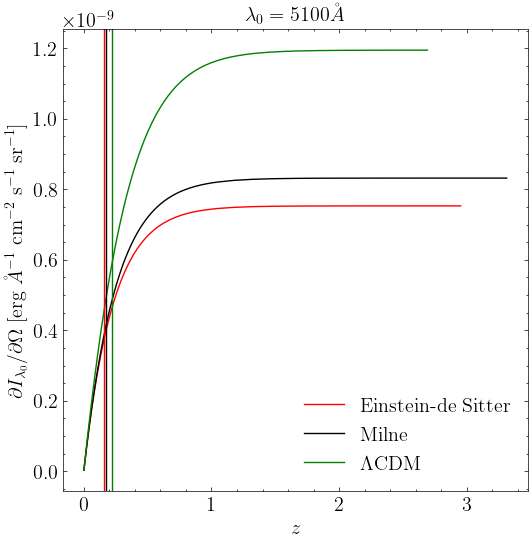
\includegraphics[width=\textwidth]{flux_univers}
                \caption{Illustration e la méthode de calcul, barres verticales indiquent 
                la position de $z_{\text{median}}$ comme le redshift où l'intensité atteint la 
        moitié de son maximum. L'intégrale est calculé jusqu'à ce qu'un plateau soit atteint.}
                \label{fig:flux}
        \end{subfigure}
        ~
        \begin{subfigure}[t]{0.45\textwidth}
                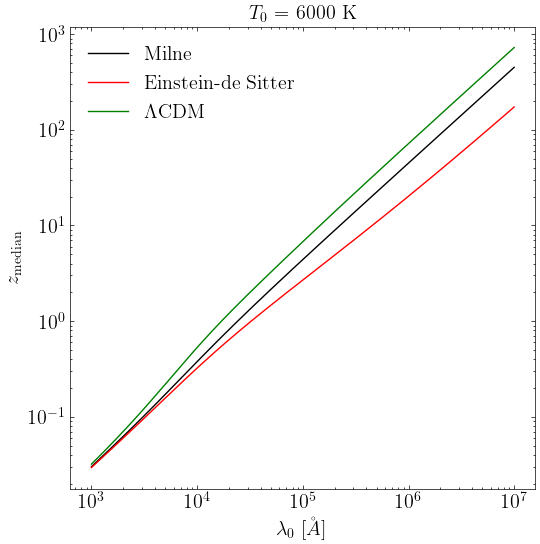
\includegraphics[width=\linewidth]{z_median_univers}
                \caption{Redshift median attendu dans un interval du spectre 
                électromagnétique.}
                \label{fig:z_median}
        \end{subfigure}
\end{figure}

On a utilisé les résultats de la collaboration Planck pour l'univers $\Lambda$CDM:
\begin{table}[H]
        \centering
        \begin{tabular}{cc}
                \toprule
                $h$ & 0.676 \\
                $\Omega_{0m}$ & 0.309\\
                $\Omega_{0r}$ & 0 \\
                $\Omega_{0\Lambda}$ & 0.679\\
                \bottomrule
                
        \end{tabular}
        \caption{Paramètres de $\Lambda$CDM}
        \label{tab:LCDMparam}
\end{table}
On a aussi définit les paramètres physique suivants (\cite{Wesson1991}):
\begin{table}[H]
        \centering
        \begin{tabular}{cc}
                \toprule 
                $T_0$ & $6000\, \text{K}$ \\
                $\epsilon_0 $ & $2.5 h\times 10^{8}\, L_{\odot}\, \text{Mpc}^{-3}$ \\
                $\lambda_0$ & $5100\s \angstrom$ \\
                \bottomrule 
        \end{tabular}
        \caption{Paramètres physiques, où $\epsilon_0 = n_0L_0$ est la densité 
        d'énergie lumineuse.}
        \label{tab:PhysParam}
\end{table}
%L'approximation $w\simeq 0$ (équation d'état) est assez bonne pour les résultats de Planck.

\subsection{Discussion}
On observe que les longueur d'onde plus énergétique ont un redshift médian beaucoup plus petit que les 
longueurs d'ondes plus rouge. De ce fait, une grande partie des emissions dans l'infrarouge 
proviennent du jeune Univers, ce qui est confirmé par les observations (CMB).

Les approximations utilisées sont les suivantes:
\begin{enumerate}
        \item On suppose que chaque objets est un corps noir
        \item On suppose que la température moyenne $T_0$ de chaque objet est constante 
                en fonction du redshift (ce qui n'est pas cohérent avec les modèles d'évolution 
                des étoiles).
        \item On a supposé un univers plat, ce qui n'est pas nécessairement le cas
        \item Notre calcul dépend de la cosmologie choisie, de façon plus importante pour 
                les redshift médian dans l'infrarouge. On a donc supposé que les trois cosmologies 
                choisies étaient de bon candidat pour comparer avec les observations.
        
\end{enumerate}



\section{Homogénéité de l'Univers}
On considère un échantillon de galaxies du sondage BOSS dans le cône:
\begin{enumerate}
        \item $0.0001 \leq z \leq 1$
        \item $156^{\circ} \leq \text{ra} \leq 160^{\circ}$
        \item $27^{\circ} \leq \text{dec} \leq 33^{\circ}$
\end{enumerate}
Ceci équivaut à plus de 15,000 galaxies, dispersés de façon inégale selon le redshift.
\begin{figure}[H]
        \centering
        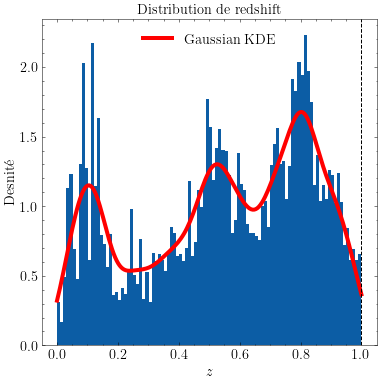
\includegraphics[width=0.5\textwidth]{redshift_dist}
        \caption{}
        \label{fig:RedshiftDist}
\end{figure}
On tient compte de cette distribution en ajustant un Kernel Density Estimator gaussien
sur le distribution. Ainsi, on peut associer un poids à chaque galaxie selon son redshift:
\begin{equation}\label{eq:poids} 
        w(z) = \frac{(P_{\text{KDE}}(z))^{-1}}{\displaystyle\int_0^{1}(P_\text{KDE}(z))^{-1}}
\end{equation} 


\subsection{Nombre de voisins dans une sphère de rayon $r$}
Une première approche pour modéliser l'excès de la densité numérique par rapport à 
un processus de Poisson est de moyenner sur chaque galaxie 
le nombre de voisins trouvés dans une 
sphère de rayon $r$. Le comportement attendu est que le nombre de galaxie augmente selon 
$r^3$ pour un processus de Poisson. Ainsi, une mesure d'homogénéité est 
\[
        \mathcal{N}(< r) = \frac{\langle N_{\text{D}}(<r)\rangle_w}{
        \langle N_{\text{R}}(<r)\rangle}
\]
ou l'indice $w$ indique la moyenne pesée avec les poids normalisés de l'équation 
\eqref{eq:poids} et 
où $N_{\text{R}}(<r)$ est le nombre de voisins dans un catalogue synthétique 
avec une distribution de densité uniforme. On s'attend à ce que 
$\mathcal{N}(<r) \rightarrow 1$ lorsque la distribution 
devient homogène à l'échelle sondée.

Pour déterminer la distance comobile $r$ (on suppose un Univers de courbure nulle), on utiliser 
la cosmologie $\Lambda \text{CDM}$ avec les résultats de la collaboration Planck (table \ref{tab:LCDMparam}).


Pour améliorer la confiance du calcul, on crée 100 catalogues synthétiques pour obtenir 
des statistiques sur $\mathcal{N}(<r)$. Finalement, chaque réalisation du calcul est obtenu 
à l'aide de 5000 galaxies choisies aléatoirement du catalogue.

\begin{figure}[H]
        \centering
        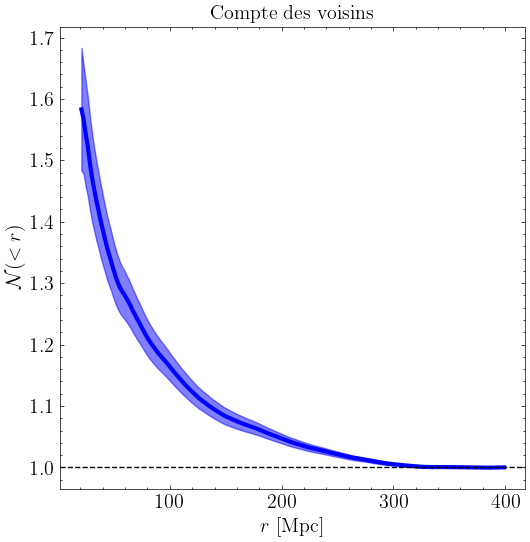
\includegraphics[width=0.5\textwidth]{coorelation_count-in-sphere}
        \caption{100 réalisations du compte de nombre de voisins pour 5000 objets 
        sélectionnés du catalogue}
        \label{fig:CountInSphere}
\end{figure}

\subsection{Fonction de covariance $\xi(r)$}

On définit la fonction d'covariance $\xi(r)$ comme l'amplitude de la tendance 
aux galaxies de s'agglomérer \cite{Peebles1980}:
\[
        dP = \bar{n} (1 + \xi(r)) dV
\]
où $dP$ mesure la probabilité de trouvé un voisin à une distance $r$ dans un un volume $dV$. 
Ainsi, $\xi(r)$ mesure l'excès de probabilité par rapport à un processus de Poisson (où 
la probabilité est fixe $dP_{\text{Poisson}} = \bar{n}dV$). En pratique, on peut définir 
l'estimateur de Davis et Peebles basé sur l'histogramme des distances de chaque paires \cite{Davis1983}:
\begin{equation}\label{eq:DavisPeebles} 
        \hat{\xi}_{DP}(r) + 1 = \frac{\bar{n}_R}{\bar{n}_D}\frac{\langle N_{\text{D}}(r) \rangle_w}{
        \langle N_{\text{R}}(r) \rangle}
\end{equation} 
où $N_{\text{D}}$ est le nombre de voisins d'une galaxie dans une coquille à un rayon $r$ 
d'épaisseur $dr$. Certains estimateur ont été introduis avec une erreur statistique plus 
basse. On définit ainsi l'estimateur d'Hamilton \cite{Hamilton1983}:
\begin{equation}\label{eq:Hamilton} 
        \hat{\xi}_H(r) + 1 =  \frac{\expval{N_D(r)}_w \expval{N_R(r)}}{\expval{N_{DR}(r)}^2}
\end{equation} 
où $N_{DR}$ est l'histogramme des distances entre les deux catalogues. Finalement, 
on introduit l'estimateur de Landy-Szalay \cite{Landy1993}
\begin{equation}\label{eq:Landy} 
        \hat{\xi}_{LS}(r) + 1 = \frac{1}{\expval{N_R}} \left[ 
                \expval{N_D}_w \left( \frac{\bar{n}_R}{\bar{n}_D} \right)^{2}
                - 2 \expval{N_{DR}} \left( \frac{\bar{n}_R}{\bar{n}_D} \right)
                + \expval{N_R}
        \right] 
\end{equation} 


\begin{figure}[H]
        \centering
        \begin{subfigure}[t]{0.3\textwidth}
                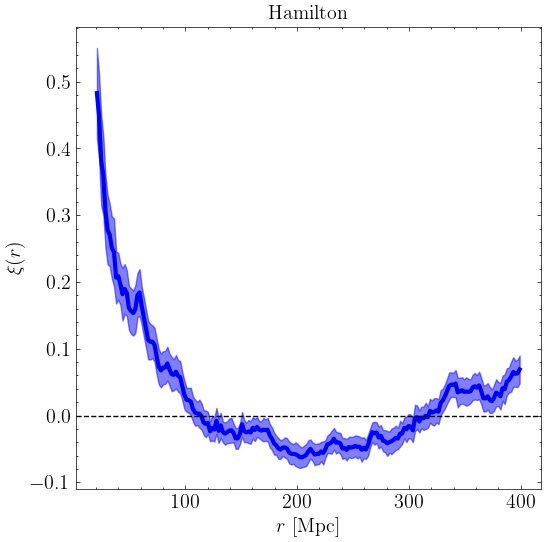
\includegraphics[width=\textwidth]{coorelation_Hamilton}
                \caption{100 réalisations de la formule \eqref{eq:Hamilton} pour 5000 objets.}
                \label{fig:Hamilton}
        \end{subfigure}
        ~
        \begin{subfigure}[t]{0.3\textwidth}
                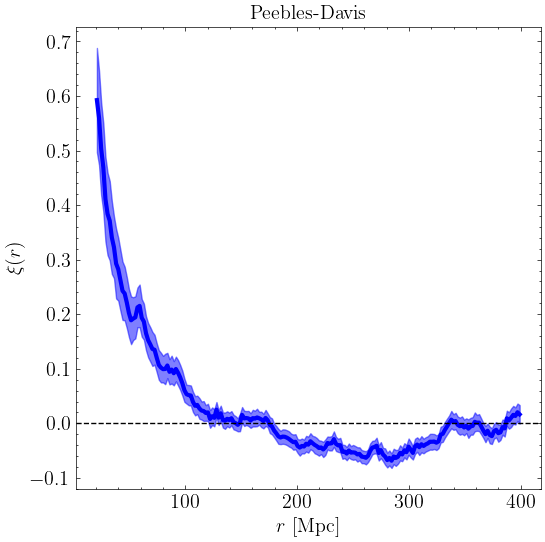
\includegraphics[width=\textwidth]{coorelation_Peebles-Davis}
                \caption{100 réalisations de la formule \eqref{eq:DavisPeebles} pour 5000 objets.}
                \label{fig:Peebles}
        \end{subfigure}
        ~
       \begin{subfigure}[t]{0.3\textwidth}
                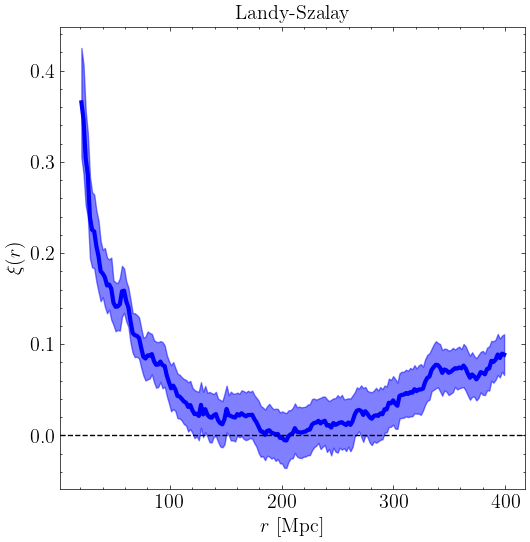
\includegraphics[width=\textwidth]{coorelation_Landy-Szalay}
                \caption{100 réalisations de la formule \eqref{eq:Landy} pour 5000 objets.}
                \label{fig:Landy}
        \end{subfigure}

\end{figure}


\subsection{Discussion}
\subsubsection{Résultats}
L'Univers devient homogène lorsque la fonction de covariance tend vers 0. Selon nos trois estimateurs, 
ceci survient autour de 
\[
        \boxed{r \sim 200\, \text{Mpc}}
\]
qui est la moyenne l'estimé provenant du compte de voisins et les fonctions de covariances (qui predisent 
autour de $r \sim 100\, \text{Mps}$).

\subsubsection{Biais}
\begin{enumerate}
        \item On assume une cosmologie avec courbure nulle;
        \item On assume le modèle $\Lambda \text{CDM}$, donc l'échelle de distance dépend de notre choix pour $h$ et 
                le paramètres de densité $\Omega_{0m}$;
        \item Notre estimateur dépend fortement de la qualité des catalogues synthétiques, donc le nombre de points utilisés 
                dans le catalogue influence le bruit intrinsèque (de Poisson) dans chaque bin de l'histogramme;
        \item Une source de bruit importante pour le redshift est la vitesse propre des galaxies, et ce bruit n'est 
                pas pris en compte dans notre analyse;
        \item Notre analyse suppose que l'Univers est \textit{statique}, en ce sens qu'on ne suppose pas de modèle 
                d'évolution des galaxies en fonction du redshift. Une analyse plus poussée devrais prendre en 
                compte cette distribution pour isoler 
                la correlation spatial des galaxies.
\end{enumerate}
Notons que notre analyse n'est pas influencée par la fenêtre de sélection du catalogue puisque le catalogue synthétique 
possède la même fenêtre de sélection.



\section{Les unités en cosmologie}
On considère les unités naturelles
\[
        c = \hbar = k_B = 1
\]
Dans ce système d'unité, le temps et les distances sont en cm, de même que l'inverse de la masse $\text{m}^{-1}$, 
et l'inverse de l'énergie $\text{E}^{-1}$. On trouve les facteurs de conversions suivants
\begin{align*}
        1\, \text{s} &\mapsto  29,979,245,800 \,\, \text{cm} \\
        1\, \si{\electronvolt^{-1}} &\mapsto \frac{\hbar c }{\si{\electronvolt}}= 1.973 \times 10^{-5} \,\, \text{cm} \\
        1\, \text{g}^{-1} &\mapsto \frac{\hbar}{c} \text{g}^{-1} = 3.518 \times 10^{-38} \,\, \text{cm}   
\end{align*}
\subsection{$H_0$}
\[
        H_0 \equiv 100 h \s \si{\kilo\meter \per \second \per \mega \parsec}
\]
\subsubsection{Conversion en $\si{\electronvolt}$}
\[
        H_0 \mapsto \hbar H_0 \simeq 2.13h \times 10^{-33}\,\, \si{\electronvolt}
\]

\subsubsection{Conversion en $\textmd{Mpc}^{-1}$}\label{sec:TailleUnivers}
\[
        H_0 \mapsto \frac{H_0}{c} \simeq 3.34h \times 10^{-4} \,\, \text{Mpc}^{-1}
\]
\subsubsection{Conversion en $\textmd{Gyr}^{-1}$}
\[
        H_0 \simeq 0.10h \,\, \text{Gyr}^{-1}
\]

\subsubsection{Conversion en $\textmd{m}\, \textmd{s}^{-2}$}
\[
        H_0 \mapsto H_0 c \simeq 9.72h \times 10^{-10}\,\, \text{m}\,\,\text{s}^{-2}
\]

\subsection{Taille caractéristique}
L'Univers devient homogène à la distance caractéristique où l'accélération gravitationnelle de Newton 
d'un amas de galaxie (typiquement $10^{15} M_\odot$) 
est égale au taux d'expansion de l'univers au temps présent. 
\[
        \frac{GM}{R^2} = H_0 c \implies R = \sqrt{\frac{GM}{H_0 c}} \simeq 37.9h^{-1/2} \,\, \text{Mpc}
\]

\subsection{$\rho_{\textmd{crit}}$}
La densité critique est
\[
        \rho_{\text{crit}} = \frac{3 H_0^2}{8 \pi G}
\]

\subsubsection{Conversion en $\si{\gram \per\centi\meter^{3}}$}
\[
        \rho_{\text{crit}} = 1.88h^{2} \times 10^{-29}\,\, \text{g} \,\, \text{cm}^{-3}
\]

\subsubsection{Conversion en $\si{\giga \electronvolt^{4}}$}
\[
        \rho_{\text{crit}} \mapsto \frac{c}{\hbar} (\hbar c)^4 \rho_{\text{crit}}
        \simeq 8.096 h^2 \times 10^{-47}\,\, \si{\giga\electronvolt^{4}}
\]

\subsubsection{Conversion en $\si{\electronvolt \per \centi\meter^{3}}$}
\[
        \rho_{\text{crit}} \mapsto c^2 \rho_{\text{crit}} \simeq 1.05 h^2 \times 10^{4}\,\, 
        \si{\electronvolt}\, \text{cm}^{-3}
\]

\subsubsection{Conversion en \textmd{protons}/$\textmd{cm}^{3}$}
\[
        \rho_{\text{crit}} \mapsto \frac{\rho_{\text{crit}}}{m_p} \simeq 
        1.123h^2\times 10^{-5}\,\, \text{protons}\,\,\text{cm}^{-3}
\]

\subsubsection{Conversion en $M_\odot / \textmd{Mpc}^{3}$}
\[
        \rho_{\text{crit}} = 2.78h^2 \times 10^{11}\,\, M_\odot\,\, \text{Mpc}^{-3}
\]


\section{Le rayon de Schwarzschild}
Pour estimer la masse de l'Univers, on utilise la densité critique $\rho_{\text{crit}}$ 
et le rayon de Hubble (distance par rapport à l'observateur à partir de laquelle 
la vitesse de récession dépasse la vitesse de la lumière -- aussi nommé horizon cosmique)
\[
        R_H \equiv \frac{c}{H_0} \simeq 2998h^{-1}\,\, \text{Mpc}
\]
%On peut estimer la masse de l'univers en utilisant la fraction de masse 

\[
        M =  \rho_{\text{crit}} \frac{4 \pi R_H^{3}}{3} = \frac{c^3}{2GH_0} 
       \simeq 3.132  h^{-1} \times 10^{22}\, M_\odot
\]
C'est la formule de Hoyle-Carvalho.
Le rayon de Schwarzschild est donc:
\[
        r_s \equiv \frac{2 G M}{c^2} =  R_H
\]

\subsection{Horizon}
On suppose que le tenseur de stress-énergie tombe à zéro à l'extérieur de l'horizon cosmique.
En principe, ceci implique qu'un élément de matière test ressent une force d'attraction gravitationnelle 
seulement vers la direction intérieur de l'Univers (vers le centre de l'Univers, qui se situe à la 
position de l'observateur $\mathcal{O}$ dans notre expérience de pensée). Ainsi, on s'attendrait 
à voir le redshift de ces galaxies vers le bleu plutôt que le rouge. Il est évident que ce 
n'est pas ce qu'on observe.

\subsection{Différentes cosmologie}
Le rayon de Schwarzschild dépend de la cosmologie choisie. Dans un espace courbe, le paramètre de densité 
critique $\Omega_0 \not= 1$. Ainsi, lorsque $k > 1$, $\Omega_0 > 1$ et le rayon de Schwarzschild est généralement 
plus grand que le rayon cosmique. De la même façon, un univers ouvert aura un rayon de Schwarzschild plus 
petit que le rayon cosmique.



\section{La métrique}
\subsection{Redéfinir $\pi$}
Existe-t-il un univers où le ratio entre le rayon et la circonférence est constant et 
égal à 3? Pour répondre à la question, on considère un univers homogène et 
isotropique définit par la métrique suivante: 
\[
        ds^2 = \frac{dr^2}{1 - kr^2} + r^2d\Omega^2
\]
où $k \in \{-1, 0, 1\}$ et $r \in [0,1[$ est une coordonnée affine. 
La circonférence d'un cercle est défini par
\[
        C = \oint_\gamma \sqrt{ds^2} = 2 \pi R
\]
où $\gamma$ est la trajectoire avec $r=R$, $\theta=\pi/2$ et 
$\phi \in [0, 2 \pi]$. Le 
rayon du cercle, quant à lui, est définit comme
\[
        R_c = \int_0^R \frac{dr'}{\sqrt{1 - kr'^2}}
\]
Ainsi, on obtient les trois ratio suivant (pour les différentes valeurs de $k$):
\[
        \frac{C}{R_c} = \left\{ 
\begin{matrix}
        2 \pi, & k = 0 \\[3ex]
        \dfrac{2\pi R}{\arcsin R} < 2 \pi, & k = 1 \\[3ex]
        \dfrac{2 \pi R}{\sinh^{-1} R} > 2 \pi, & k = -1

\end{matrix}
        \right.
\]
Pour un espace fermé ($k=1$), le rapport entre la circonférence et le rayon varie 
en fonction de la coordonnée affine du rayon. Dans ce cas, il serait possible de 
redéfinir $\pi = 3$. Examinons l'expansion de Taylor de l'expression pour $k=1$ autour 
de $R = 0$:
\[
        \frac{C}{R_c} \simeq \frac{2 \pi R}{R + \dfrac{R^3}{6} + \mathcal{O}(R^5)}
        \simeq 2 \pi \left(  1 - \frac{R^2}{6} - \mathcal{O}(R^4)\right)
\]
Pour redéfinir $\pi = 3$, alors le cercle de référence 
doit être crée à la coordonnée affine
\[
        R^* \simeq 0.532
\]
Dans la perspective de cet univers, le rapport circonférence sur le rayon suit la loi
\[
        \frac{C}{R_c} \simeq 6 \left( 1 - \frac{(R - R^*)^3}{6|R - R^{*}|} -
                \mathcal{O}\left(\frac{(R - R^{*})^{5}}{|R - R^{*}|}\right) \right),
\]

Donc, la réponse est oui, de façon pratique on peut redéfinir $\pi = 3$ dans un 
univers fermé (de courbure positive) en utilisant un cercle de référence avec un rayon 
de coordonnée affine $R^{*} \simeq 0.532$. Ceci est en définissant $\pi$ comme la moitié 
du ratio circonférence-rayon.

Toutefois, \textbf{il n'existe pas d'univers où le ratio circonférence sur rayon est constant 
où} $\pi \not= 3.14159...$. Le ratio est constant seulement dans un univers Euclidien où 
$\pi$ ne peut pas prendre une valeur différente de celle connue. C'est à dire que 
\[
        \pi \equiv \int_{-1}^1 \frac{d\xi}{\sqrt{1 - \xi^2}}
\]
qui est basé sur la métrique $ds^2 = dx^2 + dy^2$ 
avec la condition $x^2 + y^2 = 1$. En ce sens, la valeur de la constante $\pi$ ne peut pas être 
changé puisque $\pi$ est une construction théorique liée à un espace Euclidien.


\subsection{\textit{Doddleson}, Ch. 2, P2}
On considère un espace Euclidienne avec des coordonnées polaires
\[
        g_{ij} =  
        \left( 
\begin{matrix}
        1 & 0 \\ 
        0 & r^2
\end{matrix}
        \right)
\]
où $i,j\, \in \, (r, \theta)$.
\subsubsection{Symboles de Christoffel}
Par définition
\[
        \Gamma_{\alpha \beta \gamma} = \frac{1}{2} \left( 
                \frac{\partial g_{\alpha \beta}}{\partial x^{\gamma}}
                - \frac{\partial g_{\beta \gamma}}{\partial x^{\alpha}}
                + \frac{\partial g_{\alpha \gamma}}{\partial x^{\beta}}
        \right)
\]
Les symétries $\Gamma_{\alpha \beta \gamma} = \Gamma_{\alpha \gamma \beta}$ et 
$\Gamma_{\alpha \beta \gamma} = - \Gamma_{\beta \alpha \gamma} = - \Gamma_{\gamma \alpha \beta}$ 
sont immédiatement apparentes. Notons que la seule dérivée non-nul est 
\[
        g_{\theta \theta ;r} = 2r
\]
De sortes que les seuls symboles de Christoffel non-nuls sont
\[
       \boxed{\Gamma^{\theta}_{\theta r} =  \Gamma^{\theta}_{r \theta} = 
       \frac{g^{\theta \theta}}{2} g_{\theta \theta ;r} = \frac{1}{r}}
\]
En utilisant la propriété d'antisymmétrie du coefficient complètement covariant, on trouve aussi
\[
        \boxed{\Gamma^{r}_{\theta \theta} = -g^{rr}\Gamma_{\theta \theta r} = -r}
\]
\subsubsection{Géodésiques}
Il est aussi possible de trouver les symboles de Christoffel en développant les équations d'Euler-Lagrange 
en terme de la coordonnée affine $\lambda$:
\[
        -\frac{d}{d\lambda} \left( \frac{\partial L}{\partial (dx^{\alpha} / d\lambda)} \right) 
        + \frac{\partial L}{\partial x^{\alpha}} = 0
\]
où le Lagrangien est définit comme la dérivée de la coordonnée affine en fonction du temps propre 
$\tau$:
\[
        L \left( x^{\alpha}, \frac{d x^{\alpha}}{d \lambda}  \right) = 
        \frac{d \lambda}{d \tau} =  
        \sqrt{ - g_{\alpha \beta } \frac{d x^{\alpha}}{d \lambda} \frac{d x^{\beta}}{d \lambda}  }
        = \sqrt{-\left( \frac{d r}{d \lambda}  \right)^{2} 
        - r^2 \left( \frac{d \theta}{d \lambda}  \right)^{2}}
\]
Ainsi,
\begin{align*}
        -\frac{d}{d\lambda} \left( \frac{\partial L}{\partial (dr / d\lambda)} \right)
        &= \frac{d}{d\lambda}\left( \frac{1}{L}\frac{d r}{d \lambda}  \right)  
        = \frac{1}{L}\frac{d }{d \tau} \left( \frac{d r}{d \tau}  \right) 
        = \frac{1}{L} \frac{d^{2}r}{d \tau^2} 
        \\
        -\frac{d}{d\lambda} \left( \frac{\partial L}{\partial (d\theta / d\lambda)} \right) 
        &= \frac{d }{d \lambda} \left( r^2\frac{d \theta}{d \tau}  \right)
        = \frac{1}{L} \left[ 2r  \left( \frac{d r}{d \tau}  \right)\left( \frac{d\theta}{d\tau} \right) 
        + r^2 \frac{d^{2}\theta}{d \tau}  \right]
        \\
        \frac{\partial L}{\partial r} 
        &= -\frac{1}{L} r\left( \frac{d \theta}{d \lambda} \right)^{2}
        \\
        \frac{\partial L}{\partial \theta} &=  0
\end{align*}
Sachant que l'équation d'une géodésique doit s'écrire
\[
        \frac{d^{2} x^{\alpha}}{d\tau^2} = -\Gamma^{\alpha}_{\beta \gamma} \frac{d x^{\beta}}{d \tau} \frac{d x^{\gamma}}{d \tau}  
\]
Alors on simplifie les équations d'Euler-Lagrange pour isoler la seconde dérivée au côté 
gauche. Pour la coordonnée $r$, on obtient (en simplifiant $1/L$)
\[
        \boxed{\frac{d^{2}r}{d \tau^{2}} = r\left( \frac{d\theta}{dr} \right)^{2}}
\]
Pour $\theta$:
\[
        \boxed{\frac{d^{2} \theta}{d \tau^{2}}  = -2 \left( \frac{1}{r} \right)\frac{d r}{d \tau} \frac{d \theta}{d \tau}  }
\]
On remarque qu'on obtient bien les coefficients de Christoffel de la section précédentes en tenant 
compte du fait que le facteur 2 apparaissant devant $r^{-1}$ vient de la contribution de deux termes:
$\Gamma^{\theta}_{r\theta}$ 
et $\Gamma^{\theta}_{\theta r}$.



%\subsection{\textit{Hartle}, exercice 2, ch. 2}
%Supposant que l'on puisse se situer sur la surface du Soleil et qu'on répéter l'expérience 
%de Gauss pour mesurer les angles d'un triangle. La différence entre la somme des angles 
%mesurées $\sum \alpha_i$ et la somme attendu pour un espace Euclidien $\pi$ est 
%\[
        %\sum \alpha_i - \pi \simeq \frac{A_{\triangle}}{R_\odot^{2}} 
        %\left( \frac{GM_\odot}{R_\odot c^2} \right)
%\]
%Le premier facteur est un effet purement géométrique (le Soleil est une sphère en première 
%approximation), alors que le second facteur est une correction approtée par la relativité générale.

%En supposant qu'on répète l'expérience de Gauss, on mesure l'angle du triangle entre les monts 
%Brocken, Hohenhagen et Inselberg. Les distances entre ces montagnes sont $69\, \text{km}$, 
%$85\, \text{km}$ et $107\, \text{km}$. En utilisant la formule de Héron, 
%\[
        %A_\triangle \simeq 2929\, \text{km}^2
%\]
%De sortes que
%\[
        %\frac{A_\triangle}{R^2} \simeq 
%\left\{ 
%\begin{matrix}
        %6.05 \times 10^{-9}, & R_\odot \\
        %7.20 \times 10^{-5}, & R_\oplus
%\end{matrix}
%\right.
%\]
%et
%\[
        %\frac{GM_\odot}{c^2R_\odot} \simeq 
%\left\{ 
%\begin{matrix}
        %2.12 \times 10^{-6}, & R_\odot \\
        %6.95 \times 10^{-10}, & R_\oplus
%\end{matrix}
%\right.
%\]
%Pour une déviation égale à
%\[
        %\sum \alpha_i - \pi \simeq 
%\left\{ 
%\begin{matrix}
        %1.29 \times 10^{-14}, & R_\odot \\ 
        %5.01 \times 10^{-14}, & R_\oplus
%\end{matrix}
%\right.
%\]
%On remarque que dans les deux cas, la déviation est similaire mais la source de cette déviation 
%est différente. Pour le Soleil, l'effet gravitationnel est beaucoup plus important que l'effet géométrique.


%\bliography{../bibfile}
\bibliography{bibfile.bib}
\bibliographystyle{plain}

%\begin{thebibliography}{9}
        %\bibitem{StabellRefsdal}
        %Stabell, R., \& Refsdal, S. (1966). Classification of General Relativistic World Models. Monthly Notices of the Royal Astronomical Society, 132(2), 379–388. \url{https://doi.org/10.1093/mnras/132.2.379}
        %\bibitem{Wesson91}
        %Wesson, P. S. (1991). Olbers’s paradox and theectral intensity of the extragalactic background light. In The Astrophysical Journal (Vol. 367). \url{https://doi.org/10.1086/169638}

        %\bibitem{Wesson87}
        %Wesson, P. S., Valle, K., \& Stabell, R. (1987). The extragalactic background light and a definitive resolution of Olbers’s paradox. The Astrophysical Journal, 317, 601. \url{https://doi.org/10.1086/165306}
        
%\end{thebibliography}

\end{document}

